\documentclass[a4paper]{article}
\usepackage{xeCJK}
\usepackage{geometry}
\geometry{left=2.5cm,right=2.5cm,top=3cm,bottom=3cm}
\title{Algorithm Homework 3}
\author{龙肖灵 \\Xiaoling Long\\Student ID.:81943968\\email:longxl@shanghaitech.edu.cn}
\usepackage{graphicx}
\usepackage[colorlinks,linkcolor=red]{hyperref}
\usepackage{amsmath, amsthm, amssymb}
%\usepackage{subfloat}
\usepackage{float}
\usepackage{setspace}
\usepackage{enumerate}
\usepackage{colortbl}
\usepackage{multirow}
\usepackage{tikz}
\usetikzlibrary{graphs}
\usetikzlibrary{quotes}
\usepackage{pgf}
\usepackage{listings}
\usepackage{subfigure}
%\usepackage[usenames,dvipsnames,svgnames,table]{xcolor}
\newtheorem{prop}{Proposition}
\usepackage{ulem}

\newenvironment{solution}
  {\renewcommand\qedsymbol{$\blacksquare$}\begin{proof}[Solution]}
  {\end{proof}}

\renewcommand{\baselinestretch}{1.2}

\definecolor{light-gray}{gray}{0.7}
\usepackage{indentfirst}
\lstset{% general command to set parameter(s)
basicstyle=\ttfamily,frame=tlb,backgroundcolor=\color{light-gray},breaklines}

\begin{document}
\maketitle

\section*{Problem 1}
\paragraph{}
Run the Ford-Fulkerson algorithm on the flow network in the figure below, and show the residual network
after each flow augmentation. For each iteration, pick the augmenting path that is lexicographically smallest.
( e.g., if you have two augmenting path $1\to 3\to t$ and$1\to 4\to t$ , then you should choose $1\to 3\to t$, which
is lexicographically smaller than $1\to 4\to t$).
\begin{center}
  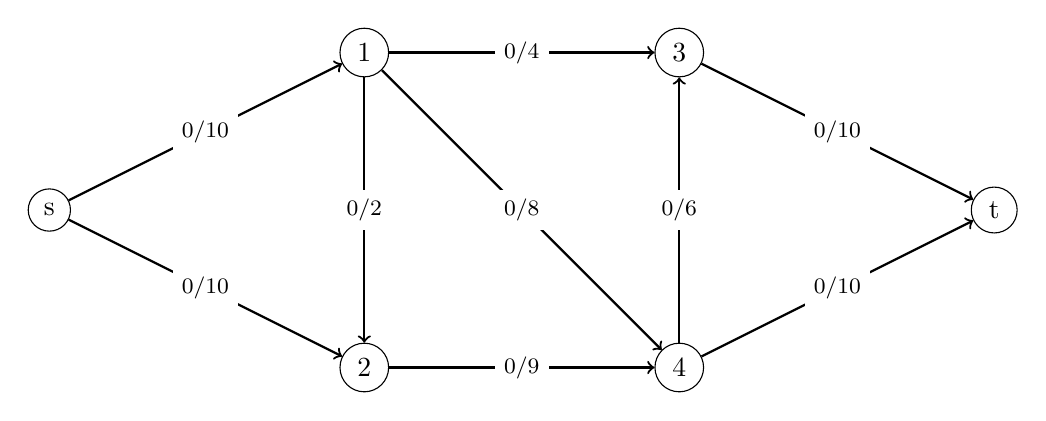
\begin{tikzpicture}[every edge quotes/.style={fill=white,font=\footnotesize}]


    \node[circle,draw]         (s) at (-6, 0)              {s};
    \node[circle,draw]         (1) at (-2, 2)           {1};
    \node[circle,draw]         (2) at (-2, -2)        {2};
    \node[circle,draw]         (3) at (2, 2)       {3};
    \node[circle,draw]         (4) at (2, -2)           {4};
    \node[circle,draw]         (t) at (6, 0)          {t};


    \draw (s) edge["0/10", ->,thick]  (1);
    \draw (s) edge["0/10", ->,thick]  (2);
    \draw (1) edge["0/2", ->,thick]  (2);
    \draw (1) edge["0/4", ->,thick]  (3);
    \draw (1) edge["0/8", ->,thick] (4);
    \draw (2) edge["0/9", ->,thick] (4);
    \draw (3) edge["0/10", ->,thick] (t);
    \draw (4) edge["0/6", ->,thick] (3);
    \draw (4) edge["0/10", ->,thick] (t);
  \end{tikzpicture}
\end{center}


\begin{solution}\ Suppose that $t$ is bigger than any other number lexicographically.
  \begin{enumerate}[1)]
    \item Select path $s\to 1\to 2\to 4 \to t$. And augment $flow=2$. Update graph.
    \begin{center}
      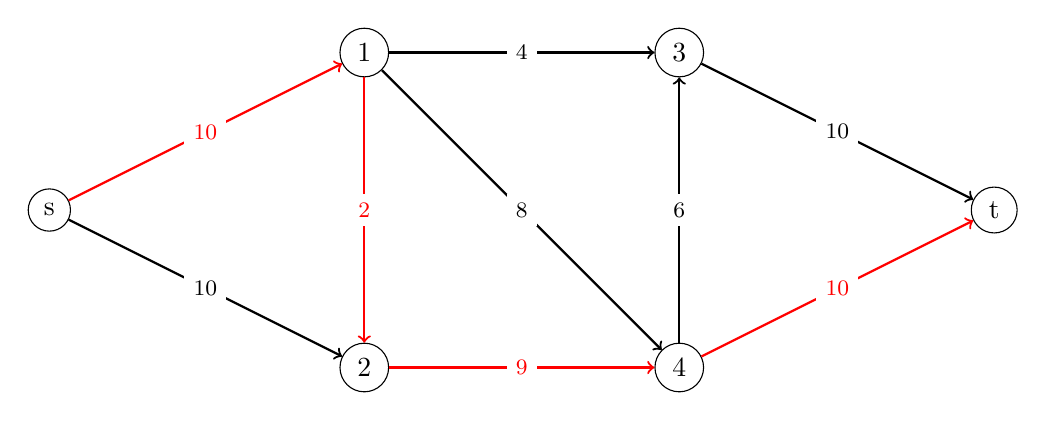
\begin{tikzpicture}[every edge quotes/.style={fill=white,font=\footnotesize}]


        \node[circle,draw]         (s) at (-6, 0)              {s};
        \node[circle,draw]         (1) at (-2, 2)           {1};
        \node[circle,draw]         (2) at (-2, -2)        {2};
        \node[circle,draw]         (3) at (2, 2)       {3};
        \node[circle,draw]         (4) at (2, -2)           {4};
        \node[circle,draw]         (t) at (6, 0)          {t};


        \draw (s) edge["10", red,->,thick]  (1);
        \draw (s) edge["10", ->,thick]  (2);
        \draw (1) edge["2",,red ,->,thick]  (2);
        \draw (1) edge["4", ->,thick]  (3);
        \draw (1) edge["8", ->,thick] (4);
        \draw (2) edge["9", red,->,thick] (4);
        \draw (3) edge["10", ->,thick] (t);
        \draw (4) edge["6", ->,thick] (3);
        \draw (4) edge["10",red, ->,thick] (t);
      \end{tikzpicture}
    \end{center}
    \begin{center}
    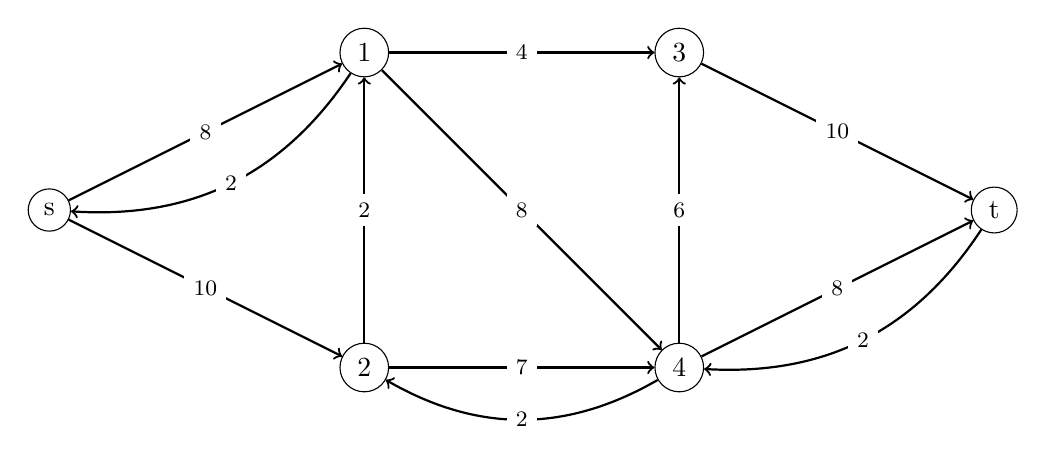
\begin{tikzpicture}[every edge quotes/.style={fill=white,font=\footnotesize}]


      \node[circle,draw]         (s) at (-6, 0)              {s};
      \node[circle,draw]         (1) at (-2, 2)           {1};
      \node[circle,draw]         (2) at (-2, -2)        {2};
      \node[circle,draw]         (3) at (2, 2)       {3};
      \node[circle,draw]         (4) at (2, -2)           {4};
      \node[circle,draw]         (t) at (6, 0)          {t};


      \draw (s) edge["8", ->,thick]  (1);
      \draw (s) edge["10", ->,thick]  (2);
      \draw (1) edge["2",bend left,->,thick]  (s);
      \draw (2) edge["2",->,thick]  (1);
      \draw (1) edge["4", ->,thick]  (3);
      \draw (1) edge["8", ->,thick] (4);
      \draw (2) edge["7",->,thick] (4);
      \draw (4) edge["2", bend left,->,thick] (2);
      \draw (3) edge["10", ->,thick] (t);
      \draw (4) edge["6", ->,thick] (3);
      \draw (4) edge["8", ->,thick] (t);
      \draw (t) edge["2",bend left, ->,thick] (4);
    \end{tikzpicture}
  \end{center}
  \item Select path $s\to 1\to 3 \to t$. And augment $flow=2+4=6$. Update graph.
  \begin{center}
  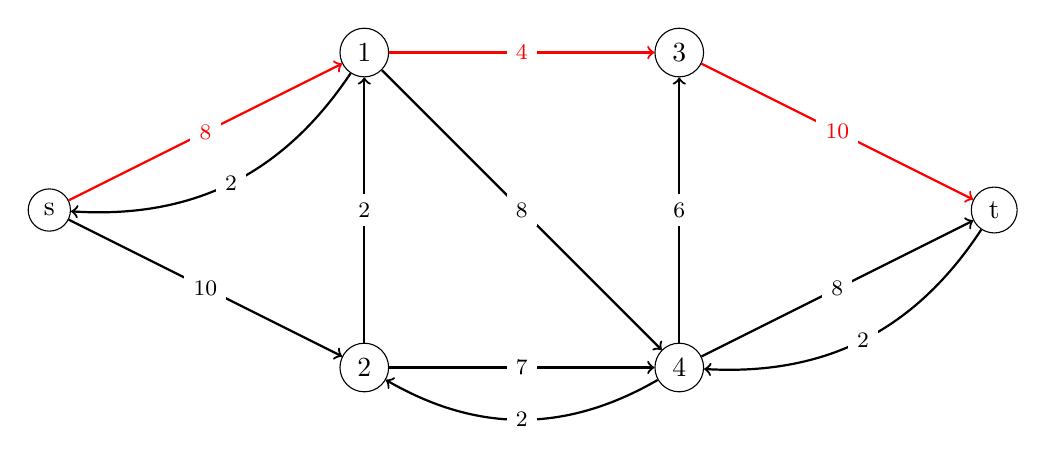
\begin{tikzpicture}[every edge quotes/.style={fill=white,font=\footnotesize}]


    \node[circle,draw]         (s) at (-6, 0)              {s};
    \node[circle,draw]         (1) at (-2, 2)           {1};
    \node[circle,draw]         (2) at (-2, -2)        {2};
    \node[circle,draw]         (3) at (2, 2)       {3};
    \node[circle,draw]         (4) at (2, -2)           {4};
    \node[circle,draw]         (t) at (6, 0)          {t};


    \draw (s) edge["8",red, ->,thick]  (1);
    \draw (s) edge["10", ->,thick]  (2);
    \draw (1) edge["2",bend left,->,thick]  (s);
    \draw (2) edge["2",->,thick]  (1);
    \draw (1) edge["4",red, ->,thick]  (3);
    \draw (1) edge["8", ->,thick] (4);
    \draw (2) edge["7",->,thick] (4);
    \draw (4) edge["2", bend left,->,thick] (2);
    \draw (3) edge["10",red, ->,thick] (t);
    \draw (4) edge["6", ->,thick] (3);
    \draw (4) edge["8", ->,thick] (t);
    \draw (t) edge["2",bend left, ->,thick] (4);
  \end{tikzpicture}
  \end{center}
  \begin{center}
  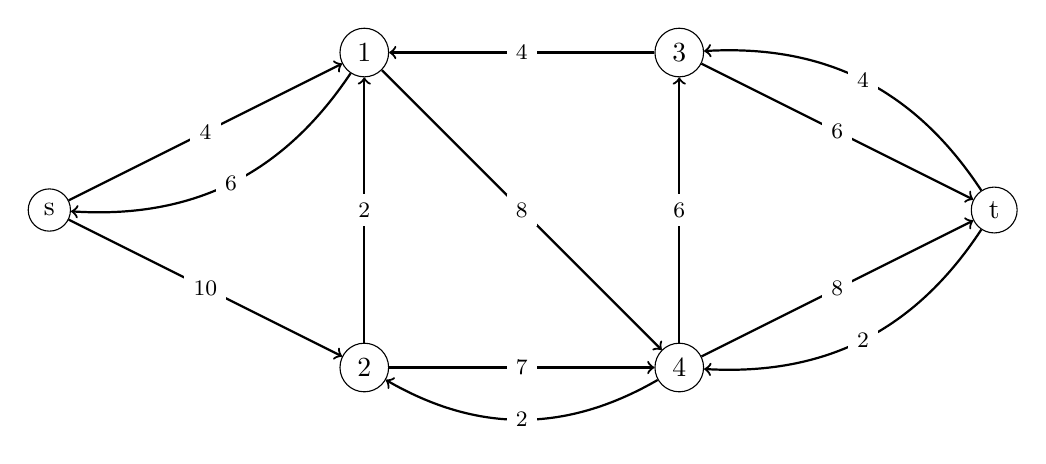
\begin{tikzpicture}[every edge quotes/.style={fill=white,font=\footnotesize}]


    \node[circle,draw]         (s) at (-6, 0)              {s};
    \node[circle,draw]         (1) at (-2, 2)           {1};
    \node[circle,draw]         (2) at (-2, -2)        {2};
    \node[circle,draw]         (3) at (2, 2)       {3};
    \node[circle,draw]         (4) at (2, -2)           {4};
    \node[circle,draw]         (t) at (6, 0)          {t};


    \draw (s) edge["4", ->,thick]  (1);
    \draw (s) edge["10", ->,thick]  (2);
    \draw (1) edge["6",bend left,->,thick]  (s);
    \draw (2) edge["2",->,thick]  (1);
    \draw (3) edge["4", ->,thick]  (1);
    \draw (1) edge["8", ->,thick] (4);
    \draw (2) edge["7",->,thick] (4);
    \draw (4) edge["2", bend left,->,thick] (2);
    \draw (3) edge["6", ->,thick] (t);
    \draw (t) edge["4",bend right, ->,thick] (3);
    \draw (4) edge["6", ->,thick] (3);
    \draw (4) edge["8", ->,thick] (t);
    \draw (t) edge["2",bend left, ->,thick] (4);
  \end{tikzpicture}
  \end{center}
  \item Select path $s\to 1\to 4 \to t$. And augment $flow=6+4=10$. Update graph.
  \begin{center}
  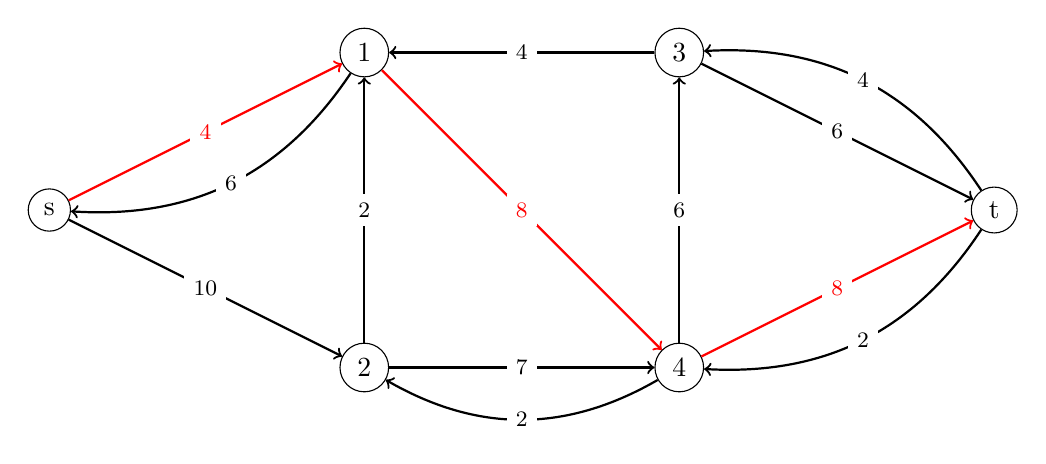
\begin{tikzpicture}[every edge quotes/.style={fill=white,font=\footnotesize}]


    \node[circle,draw]         (s) at (-6, 0)              {s};
    \node[circle,draw]         (1) at (-2, 2)           {1};
    \node[circle,draw]         (2) at (-2, -2)        {2};
    \node[circle,draw]         (3) at (2, 2)       {3};
    \node[circle,draw]         (4) at (2, -2)           {4};
    \node[circle,draw]         (t) at (6, 0)          {t};


    \draw (s) edge["4", red,->,thick]  (1);
    \draw (s) edge["10", ->,thick]  (2);
    \draw (1) edge["6",bend left,->,thick]  (s);
    \draw (2) edge["2",->,thick]  (1);
    \draw (3) edge["4", ->,thick]  (1);
    \draw (1) edge["8",red, ->,thick] (4);
    \draw (2) edge["7",->,thick] (4);
    \draw (4) edge["2", bend left,->,thick] (2);
    \draw (3) edge["6", ->,thick] (t);
    \draw (t) edge["4",bend right, ->,thick] (3);
    \draw (4) edge["6", ->,thick] (3);
    \draw (4) edge["8", red,->,thick] (t);
    \draw (t) edge["2",bend left, ->,thick] (4);
  \end{tikzpicture}
  \end{center}
  \begin{center}
  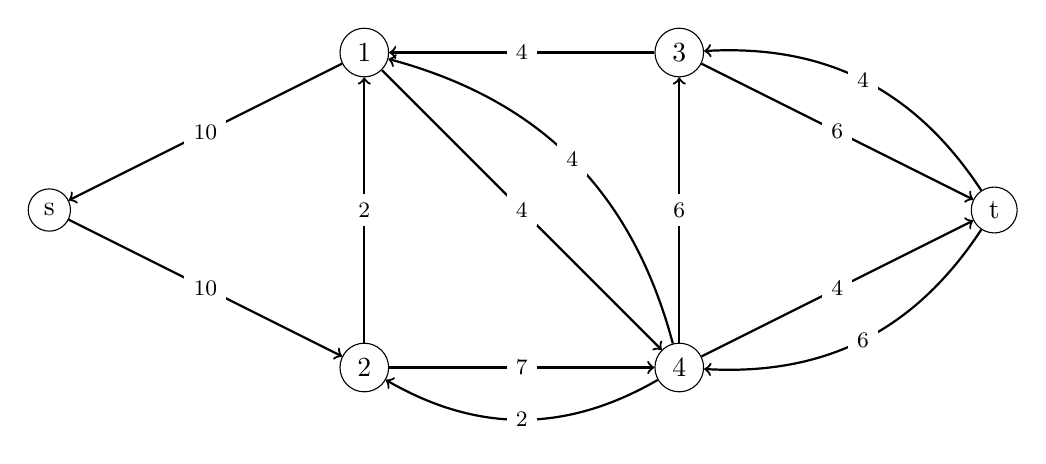
\begin{tikzpicture}[every edge quotes/.style={fill=white,font=\footnotesize}]


    \node[circle,draw]         (s) at (-6, 0)              {s};
    \node[circle,draw]         (1) at (-2, 2)           {1};
    \node[circle,draw]         (2) at (-2, -2)        {2};
    \node[circle,draw]         (3) at (2, 2)       {3};
    \node[circle,draw]         (4) at (2, -2)           {4};
    \node[circle,draw]         (t) at (6, 0)          {t};


    \draw (s) edge["10", ->,thick]  (2);
    \draw (1) edge["10",->,thick]  (s);
    \draw (2) edge["2",->,thick]  (1);
    \draw (3) edge["4", ->,thick]  (1);
    \draw (1) edge["4", ->,thick] (4);
    \draw (4) edge["4",bend right, ->,thick] (1);
    \draw (2) edge["7",->,thick] (4);
    \draw (4) edge["2", bend left,->,thick] (2);
    \draw (3) edge["6", ->,thick] (t);
    \draw (t) edge["4",bend right, ->,thick] (3);
    \draw (4) edge["6", ->,thick] (3);
    \draw (4) edge["4", ->,thick] (t);
    \draw (t) edge["6",bend left, ->,thick] (4);
  \end{tikzpicture}
  \end{center}
  \item Select path $s\to 2\to 1\to 4 \to 3 \to t$. And augment $flow=10+2=12$. Update graph.
  \begin{center}
  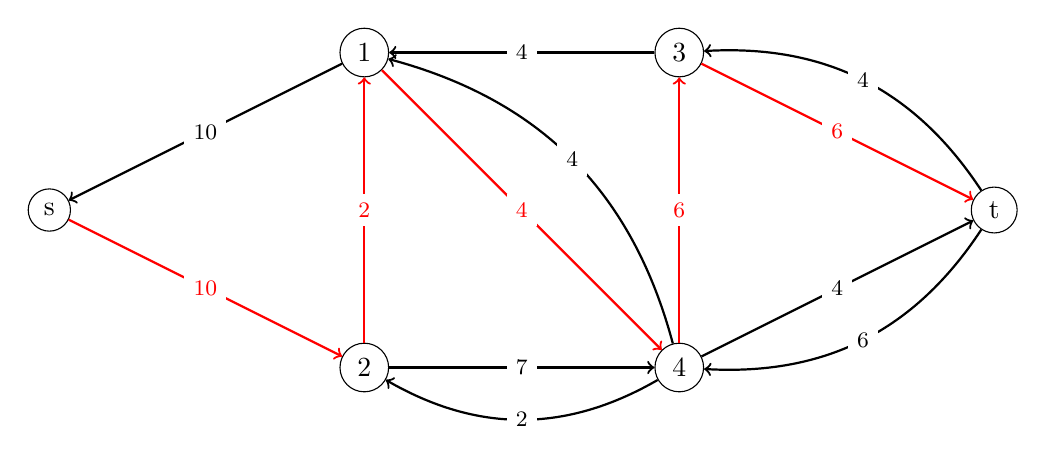
\begin{tikzpicture}[every edge quotes/.style={fill=white,font=\footnotesize}]


    \node[circle,draw]         (s) at (-6, 0)              {s};
    \node[circle,draw]         (1) at (-2, 2)           {1};
    \node[circle,draw]         (2) at (-2, -2)        {2};
    \node[circle,draw]         (3) at (2, 2)       {3};
    \node[circle,draw]         (4) at (2, -2)           {4};
    \node[circle,draw]         (t) at (6, 0)          {t};


    \draw (s) edge["10",red, ->,thick]  (2);
    \draw (1) edge["10",->,thick]  (s);
    \draw (2) edge["2",red,->,thick]  (1);
    \draw (3) edge["4", ->,thick]  (1);
    \draw (1) edge["4",red, ->,thick] (4);
    \draw (4) edge["4",bend right, ->,thick] (1);
    \draw (2) edge["7",->,thick] (4);
    \draw (4) edge["2", bend left,->,thick] (2);
    \draw (3) edge["6",red, ->,thick] (t);
    \draw (t) edge["4",bend right, ->,thick] (3);
    \draw (4) edge["6",red, ->,thick] (3);
    \draw (4) edge["4", ->,thick] (t);
    \draw (t) edge["6",bend left, ->,thick] (4);
  \end{tikzpicture}
  \end{center}
  \begin{center}
  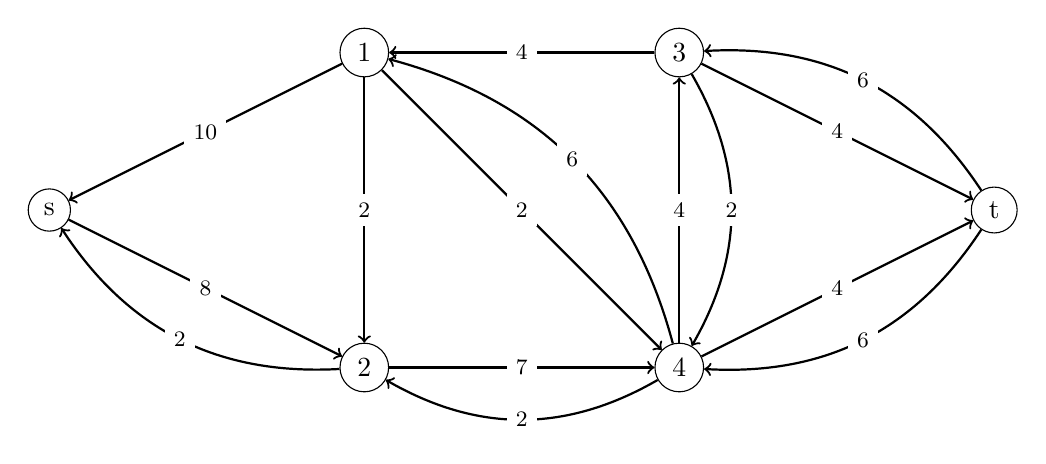
\begin{tikzpicture}[every edge quotes/.style={fill=white,font=\footnotesize}]


    \node[circle,draw]         (s) at (-6, 0)              {s};
    \node[circle,draw]         (1) at (-2, 2)           {1};
    \node[circle,draw]         (2) at (-2, -2)        {2};
    \node[circle,draw]         (3) at (2, 2)       {3};
    \node[circle,draw]         (4) at (2, -2)           {4};
    \node[circle,draw]         (t) at (6, 0)          {t};


    \draw (s) edge["8", ->,thick]  (2);
    \draw (2) edge["2",bend left, ->,thick]  (s);
    \draw (1) edge["10",->,thick]  (s);
    \draw (1) edge["2",->,thick]  (2);
    \draw (3) edge["4", ->,thick]  (1);
    \draw (1) edge["2", ->,thick] (4);
    \draw (4) edge["6",bend right, ->,thick] (1);
    \draw (2) edge["7",->,thick] (4);
    \draw (4) edge["2", bend left,->,thick] (2);
    \draw (3) edge["4", ->,thick] (t);
    \draw (t) edge["6",bend right, ->,thick] (3);
    \draw (4) edge["4", ->,thick] (3);
    \draw (3) edge["2",bend left, ->,thick] (4);
    \draw (4) edge["4", ->,thick] (t);
    \draw (t) edge["6",bend left, ->,thick] (4);
  \end{tikzpicture}
  \end{center}
  \item Select path $s\to 2\to 4 \to 3 \to t$. And augment $flow=12+4=16$. Update graph.
  \begin{center}
  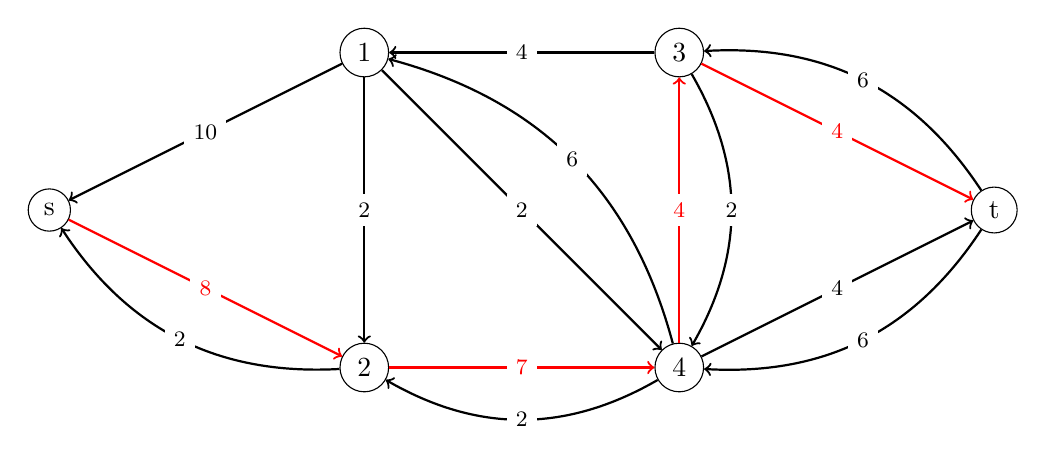
\begin{tikzpicture}[every edge quotes/.style={fill=white,font=\footnotesize}]


    \node[circle,draw]         (s) at (-6, 0)              {s};
    \node[circle,draw]         (1) at (-2, 2)           {1};
    \node[circle,draw]         (2) at (-2, -2)        {2};
    \node[circle,draw]         (3) at (2, 2)       {3};
    \node[circle,draw]         (4) at (2, -2)           {4};
    \node[circle,draw]         (t) at (6, 0)          {t};


    \draw (s) edge["8",red, ->,thick]  (2);
    \draw (2) edge["2",bend left, ->,thick]  (s);
    \draw (1) edge["10",->,thick]  (s);
    \draw (1) edge["2",->,thick]  (2);
    \draw (3) edge["4", ->,thick]  (1);
    \draw (1) edge["2", ->,thick] (4);
    \draw (4) edge["6",bend right, ->,thick] (1);
    \draw (2) edge["7",red,->,thick] (4);
    \draw (4) edge["2", bend left,->,thick] (2);
    \draw (3) edge["4", red,->,thick] (t);
    \draw (t) edge["6",bend right, ->,thick] (3);
    \draw (4) edge["4",red, ->,thick] (3);
    \draw (3) edge["2",bend left, ->,thick] (4);
    \draw (4) edge["4", ->,thick] (t);
    \draw (t) edge["6",bend left, ->,thick] (4);
  \end{tikzpicture}
  \end{center}
  \begin{center}
  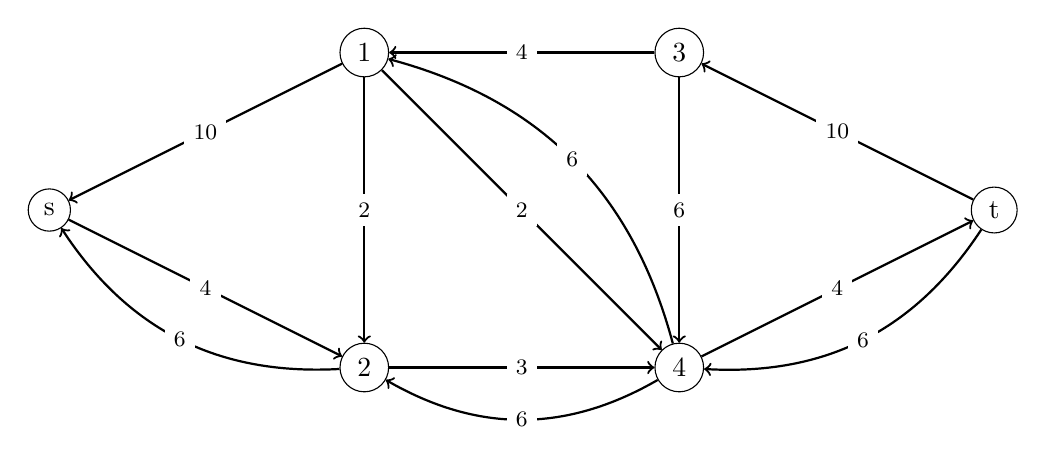
\begin{tikzpicture}[every edge quotes/.style={fill=white,font=\footnotesize}]


    \node[circle,draw]         (s) at (-6, 0)              {s};
    \node[circle,draw]         (1) at (-2, 2)           {1};
    \node[circle,draw]         (2) at (-2, -2)        {2};
    \node[circle,draw]         (3) at (2, 2)       {3};
    \node[circle,draw]         (4) at (2, -2)           {4};
    \node[circle,draw]         (t) at (6, 0)          {t};


    \draw (s) edge["4", ->,thick]  (2);
    \draw (2) edge["6",bend left, ->,thick]  (s);
    \draw (1) edge["10",->,thick]  (s);
    \draw (1) edge["2",->,thick]  (2);
    \draw (3) edge["4", ->,thick]  (1);
    \draw (1) edge["2", ->,thick] (4);
    \draw (4) edge["6",bend right, ->,thick] (1);
    \draw (2) edge["3",->,thick] (4);
    \draw (4) edge["6", bend left,->,thick] (2);
    \draw (t) edge["10", ->,thick] (3);
    \draw (3) edge["6",->,thick] (4);
    \draw (4) edge["4", ->,thick] (t);
    \draw (t) edge["6",bend left, ->,thick] (4);
  \end{tikzpicture}
  \end{center}
  \item Select path $s\to 2\to 4 \to t$. And augment $flow=16+3=19$. Update graph.
  \begin{center}
  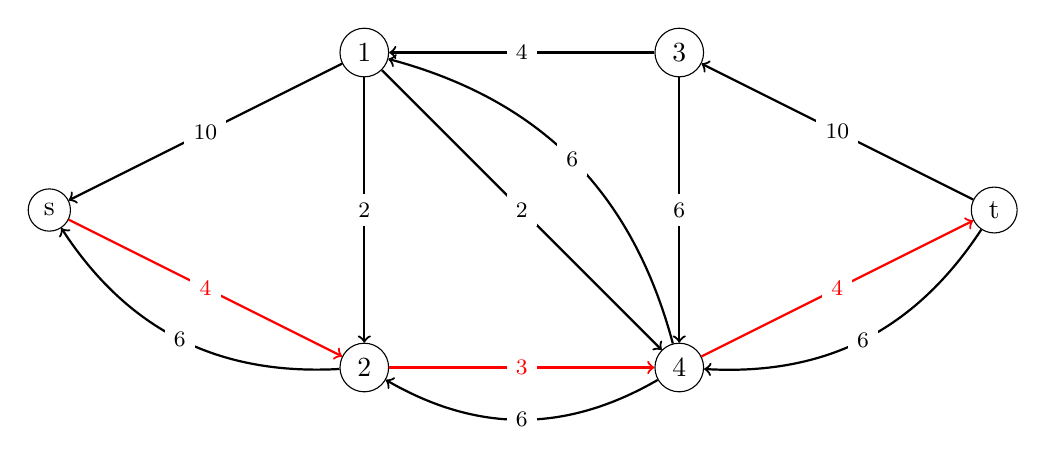
\begin{tikzpicture}[every edge quotes/.style={fill=white,font=\footnotesize}]


    \node[circle,draw]         (s) at (-6, 0)              {s};
    \node[circle,draw]         (1) at (-2, 2)           {1};
    \node[circle,draw]         (2) at (-2, -2)        {2};
    \node[circle,draw]         (3) at (2, 2)       {3};
    \node[circle,draw]         (4) at (2, -2)           {4};
    \node[circle,draw]         (t) at (6, 0)          {t};


    \draw (s) edge["4",red, ->,thick]  (2);
    \draw (2) edge["6",bend left, ->,thick]  (s);
    \draw (1) edge["10",->,thick]  (s);
    \draw (1) edge["2",->,thick]  (2);
    \draw (3) edge["4", ->,thick]  (1);
    \draw (1) edge["2", ->,thick] (4);
    \draw (4) edge["6",bend right, ->,thick] (1);
    \draw (2) edge["3",red,->,thick] (4);
    \draw (4) edge["6", bend left,->,thick] (2);
    \draw (t) edge["10", ->,thick] (3);
    \draw (3) edge["6",->,thick] (4);
    \draw (4) edge["4", red,->,thick] (t);
    \draw (t) edge["6",bend left, ->,thick] (4);
  \end{tikzpicture}
  \end{center}
  \begin{center}
  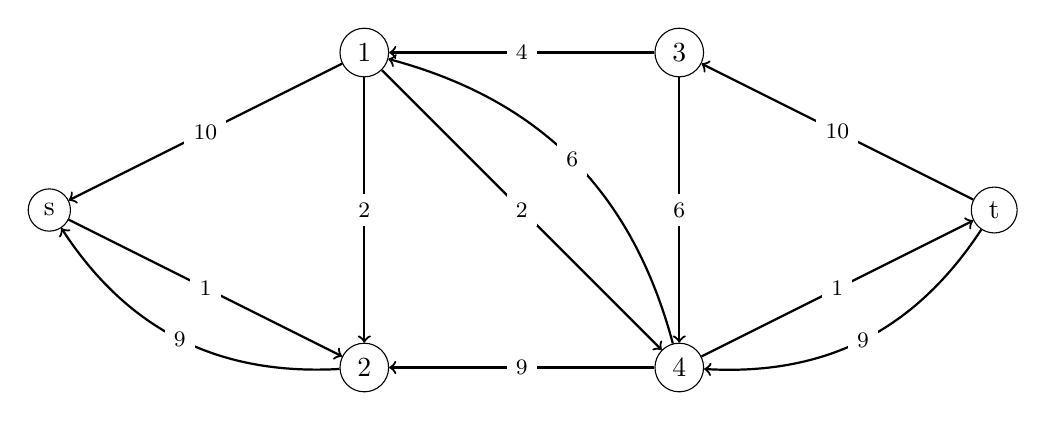
\begin{tikzpicture}[every edge quotes/.style={fill=white,font=\footnotesize}]


    \node[circle,draw]         (s) at (-6, 0)              {s};
    \node[circle,draw]         (1) at (-2, 2)           {1};
    \node[circle,draw]         (2) at (-2, -2)        {2};
    \node[circle,draw]         (3) at (2, 2)       {3};
    \node[circle,draw]         (4) at (2, -2)           {4};
    \node[circle,draw]         (t) at (6, 0)          {t};


    \draw (s) edge["1", ->,thick]  (2);
    \draw (2) edge["9",bend left, ->,thick]  (s);
    \draw (1) edge["10",->,thick]  (s);
    \draw (1) edge["2",->,thick]  (2);
    \draw (3) edge["4", ->,thick]  (1);
    \draw (1) edge["2", ->,thick] (4);
    \draw (4) edge["6",bend right, ->,thick] (1);
    \draw (4) edge["9",->,thick] (2);
    \draw (t) edge["10", ->,thick] (3);
    \draw (3) edge["6",->,thick] (4);
    \draw (4) edge["1", ->,thick] (t);
    \draw (t) edge["9",bend left, ->,thick] (4);
  \end{tikzpicture}
  \end{center}
  \item Finally, there is no path now, we can get maximum flow is $19$.
  \end{enumerate}
  Done.
\end{solution}

\section*{Problem 2}
\paragraph{}
There are $n$ staff members in a company. Each staff member belongs to a department. There are $k$
departments. Now we have to choose one staff member from each department to a company-level committee.
In this committee, there must be $m_{1}$ number of A-class staff members, $m_{2}$ number of B-class staff members,
$m_{3}$ number of C-class staff members, and $m_{4}$ number of D-class staff members (so we have $m_{1}+m_{2}+m_{3}=m_{4}=k$). We are given the list of staff members, their home departments, and their classes (A, B, C, D).
Describe an efficient algorithm to determine who should be on the committee such that the constraints are
satisfied.

\begin{solution}We can regard this problem as a maximum flow problem after do some modification as bellow.
  \begin{center}
  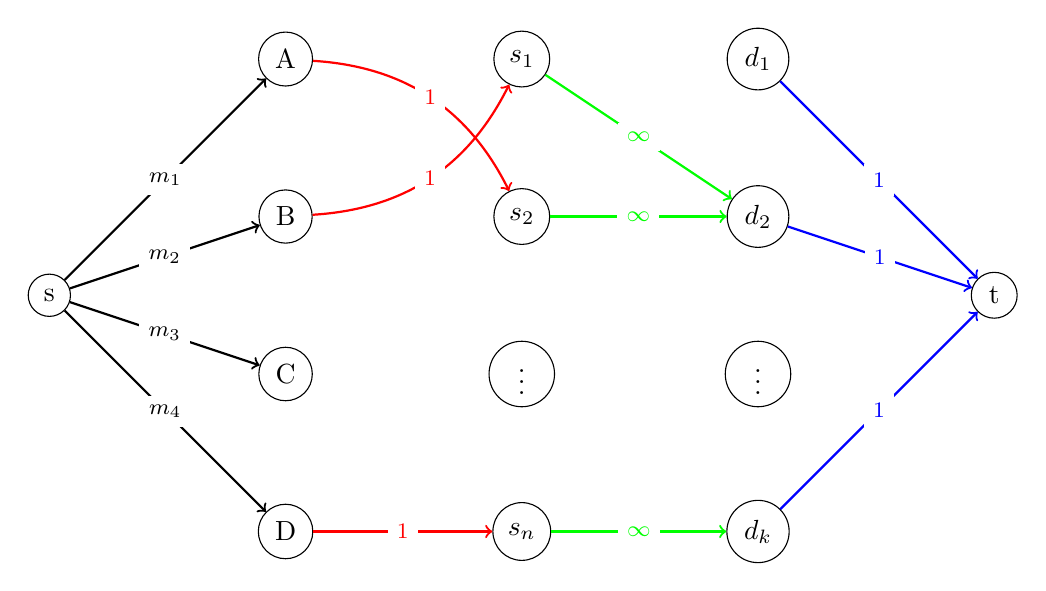
\begin{tikzpicture}[every edge quotes/.style={fill=white,font=\footnotesize}]


    \node[circle,draw]         (s) at (-6, 0)              {s};
    \node[circle,draw]         (A) at (-3, 3)           {A};
    \node[circle,draw]         (B) at (-3, 1)        {B};
    \node[circle,draw]         (C) at (-3, -1)       {C};
    \node[circle,draw]         (D) at (-3, -3)           {D};
    \node[circle,draw]         (s1) at (0, 3)           {$s_{1}$};
    \node[circle,draw]         (s2) at (0, 1)        {$s_{2}$};
    \node[circle,draw]         (s3) at (0, -1)       {$\vdots$};
    \node[circle,draw]         (sn) at (0, -3)           {$s_{n}$};
    \node[circle,draw]         (d1) at (3, 3)           {$d_{1}$};
    \node[circle,draw]         (d2) at (3, 1)        {$d_{2}$};
    \node[circle,draw]         (d3) at (3, -1)       {$\vdots$};
    \node[circle,draw]         (dk) at (3, -3)           {$d_{k}$};
    \node[circle,draw]         (t) at (6, 0)          {t};


    \draw (s) edge["$m_{1}$", ->,thick]  (A);
    \draw (s) edge["$m_{2}$", ->,thick]  (B);
    \draw (s) edge["$m_{3}$", ->,thick]  (C);
    \draw (s) edge["$m_{4}$", ->,thick]  (D);
    \draw (A) edge["$1$",red,bend left, ->,thick]  (s2);
    \draw (B) edge["$1$",red,bend right, ->,thick]  (s1);
    \draw (D) edge["$1$",red, ->,thick]  (sn);
    \draw (s1) edge["$\infty$",green, ->,thick]  (d2);
    \draw (s2) edge["$\infty$",green, ->,thick]  (d2);
    \draw (sn) edge["$\infty$",green, ->,thick]  (dk);
    \draw (d1) edge["$1$",blue, ->,thick]  (t);
    \draw (d2) edge["$1$",blue, ->,thick]  (t);
    \draw (dk) edge["$1$",blue, ->,thick]  (t);
  \end{tikzpicture}
  \end{center}
  \begin{enumerate}[(a)]
    \item Black lines: we need select $m_{i}$ $ith $-class staff number(s).
    \item Red lines: $s_{i}$ belongs to $ith$-class
    \item Green lines: $s_{i}$ lives in $d_{i}$ department.
    \item Blue lines: every department we need a commitee.
  \end{enumerate}
      So the problem become find the maximum flow in above graph. So we can solve this problme by find the maximum in above graph. If the maximum flow is $k$, then we can get the committee member satisfying the constraints. And if not, we cannot satisfy all constraints.
      And All staff member $s_{i}$ in maximum flow will be on the committee.\\
  Done.
\end{solution}

\section*{Problem 3 }
\paragraph{}
Let $G = (V, E)$ be a flow network with source $s$, sink $t$, and integer capacities. Suppose that we are
given a maximum flow in $G$.
\begin{enumerate}[1.]
  \item  Suppose that we increase the capacity of a single edge $(v, u) \in E$ by 1. Give an $O(V + E)$ time
  algorithm to update the maximum flow.
  \item  Suppose that we decrease the capacity of a single edge $(v, u) \in E$ by 1. Give an $O(V + E)$ time
  algorithm to update the maximum flow.
\end{enumerate}

\begin{solution}\
  \begin{enumerate}[1.]
    \item Add this capacity to the last residual graph.
    Do a BFS on this residual network from $s$. If find a path from $s$ to $t$, then maximum flow add 1, and the new maximum flow will augment by 1 following this path the flow value increased by 1, or not maximum flow remains. And the run time of DFS is $O(V+E)$. It can satisfy the constraint.
    \item Asume that maximum flow has no circle.(Find a maximum flow without choosing a circle).
    \begin{enumerate}[a.]
      \item Do a BFS on the last residual graph to find a path from $t$ to $u$, decrease the flow of the edge on path by 1. Update the residual graph.
      \item Do a BFS on the last residual graph to find a paht from $v$ to $s$, decrease the flow of the edge on path by 1. Update the residual graph.
      \item Decrease the flow of the edge $(v,u)\in E$ by 1. Just do $f(e^{R})=f(e^{R})-1$ on new residula graph.
      \item Do a BFS on the new residual graph. If find a path from $s$ to $t$, then update the maximum flow. The flow value remains. If not, maximum flow is on the new residual graph. And the maximum value decreased by 1.
      \item The run time of this algorithm can be $O(V+E)$, since we just do some BFS.
    \end{enumerate}
  \end{enumerate}

  Done.
\end{solution}

\section*{Problem 4}
\paragraph{}
Suppose we have an $n$-by-$m$ matrix in which each element is either 0 or 1. We know the row sums
$r=(r_{1},\cdots,r_{n})$ and the column sums $c=(c_{1},\cdots,c_{m})$ (it is guaranteed that
$\sum_{i}r_{i}=\sum_{j}c_{j}$). Design a
polynomial-time algorithm based network flow to decide whether such a matrix exists or not.
Examples: $n=m=3$ with $c = (1, 2, 0)$ and $r = (1, 1, 1)$ (answer=yes) or $r = (3, 0, 0)$ (answer=no):
\begin{table}[H]
  \centering
  \subtable{
  \begin{tabular}{|c| c |c |c}
    \multicolumn{3}{c}{Yes}&\\
    \cline{1-3}
     \cellcolor[gray]{0.8} 1&0&0&1 \\
    \cline{1-3}
    0&\cellcolor[gray]{0.8}1&0&1 \\
    \cline{1-3}
    0&\cellcolor[gray]{0.8}1&0&1 \\
    \cline{1-3}
    \multicolumn{1}{c}{1}&\multicolumn{1}{c}{2}&\multicolumn{1}{c}{0}&
  \end{tabular}
  }
  \qquad\quad
  \subtable{
  \begin{tabular}{|c| c| c |c}
    \multicolumn{3}{c}{No}&\\
    \cline{1-3}
    \cellcolor[gray]{0.8}1&\cellcolor[gray]{0.8}1&\cellcolor[gray]{0.8}1&3 \\
    \cline{1-3}
    & &&0 \\
    \cline{1-3}
    &&&0 \\
    \cline{1-3}
    \multicolumn{1}{c}{1}&\multicolumn{1}{c}{2}&\multicolumn{1}{c}{0}&
  \end{tabular}
  }
\end{table}

\begin{solution}\ To built a network based on network flow, and we can decide whether there exists a matrix or not in polynomial-time. Divide into 5 layers.
  \begin{enumerate}[1)]
    \item layer 1: Source node $s$.
    \item layer 2: $n$ row sums $R_{i}$. And edge $c(s-R_{i})=r_{i}$.
    \item layer 3: $n\times m$ nodes of elements from matrix. And for all $j$ from 1 to $m$, edge $c(R_{i}-m_{i,j})=1$.
    \item layer 4: $m$ column sums $C_{j}$. And for all $i$ from 1 to $n$, edge $c(m_{i,j}-C_{j})=1$.
    \item layer 5: Sink node $t$. Edge $c(C_{j}-t)=c_{j}$.
  \end{enumerate}
  Then solve this maximum flow problem. If we can find a maximum flow that $flow value=\sum_{i}r_{i}=\sum_{j}c_{j}$, then the matrix exists. And the elements go through will be 1, and others be 0. Or not there doesn't exist such a matrix.\\
  Done.
\end{solution}

\section*{Problem 5}
\paragraph{}
Consider a network $G = (V, E)$. In addition to having a capacity $c(u, v)$ for every edge $(u, v)$, we also have
a capacity $c(u)$ for every vertex $u$. A flow $f$ is feasible only if, in addition to the conservation constraint and
the edge capacity constraint, it also satisfies the vertex capacity constraint: $\forall v \in V, \sum_{u:(u,v)\in E}f(u,v)\le c(v)$.
Give an efficient algorithm to solve the maximum flow problem on this network.\\
Hint: You can reduce the problem to the standard maximum flow problem.
\begin{solution}We can reduce the problem to the standard maximum flow problem after process as bellow.
  \begin{enumerate}[(a)]
    \item Assume there exist a source node and a sink node.
    \item Split every node $u$ into 2 node $u_{1}$ and $u_{2}$ except source node and sink node. And there is an edge $c(u_{1},u_{2})=c(u)$.
    \item All edge $(v,u)$ become $(v,u_{1})$ and the capacity of edge $(v,u_{1})$ equals to $(v,u)$.
    \item All edge $(u,v)$ become $(u_{2},v)$ and the capacity of edge $(u_{2},v)$ equals to $(u,v)$.
    \item Then the origin problem can be solved as a standard maximum flow problem.
  \end{enumerate}
  Done.
\end{solution}

\section*{Problem 6}
\paragraph{}
Given a network $G = (V, E)$, design a polynomial time algorithm to determine whether $G$ has a unique
minimum $s-t$ cut.

\begin{solution}\ Inspirated by Problem 3.
   First find the minimum $s-t$ cut of $G$, and the edges between cut. Then for each $e$ between cut, increase the capacity of it. If there is an edge whose maximum flow in new network graph doesn't change, then the miimum cut isn't unique. Or all edge increasing change the maximum flow, means the minimum cut is unique. \\
   Actually, if an edge between cut increased by 1, and the maximum flow doesn't increase. That means the child node of this node doesn't have more capacity for flow. So this child node can get into minimum cut. The minimum cut isn't unique.\\
  Done.
\end{solution}

\end{document}
